\documentclass[0pt, a4paper]{article}
\usepackage{amsmath} % For advanced math typesetting
\usepackage{authblk} % Load authblk for multiple authors and affiliations
\usepackage{xcolor}
\usepackage{tcolorbox} %LaTeX package to custom color boxes for custom subsectioning
\usepackage{graphicx} %LaTeX package to import graphics
\usepackage{amsthm}
\usepackage{amssymb} %LaTeX package to import extra symbols
\usepackage{cancel} %LaTeX package to import cancelling

\graphicspath{{assets/}} %configuring the graphicx package

\begin{document}

\title{The Electrostatic SDK Linear Projection Project: Mathematics-I}

\author{Project Lead: Pavly Gerges}
\affil[0]{Part of the Electrostatic-Sandbox SDK, Project: ElectroNetSoft.
A generalized Math Framework for Linear Projection Algorithms, purely written in ISO/C99.}
\date{\today}

\maketitle

\section{Trigonometric identities}

\subsection{Preface}

\subsection{The use of trigonometry in game development}

\subsection{Trigonometry in Linear Projection}

\subsection{Trigonometry Basics}

\subsubsection{Unit Circle and Angles}

\subsubsection{Trigonometric Functions}

\subsubsection{Vectors and Trigonometric Functions}

\subsubsection{Polar and rectangular coordinates}

\subsubsection{Euler Angles}

\subsubsection{Basics of Quaternions}

\subsection{Analytical Trigonometry}

% Define custom subsection command with color parameter
\newcommand{\specialsubsection}[3]{
    \medskip
    \begin{tcolorbox}[colback=#3!10!white, colframe=#3!80!black, title=\textbf{#1}, sharp corners=south]
        #2
    \end{tcolorbox}
    \medskip
}

\subsubsection{Fundamentals Trigonometric identities}

This section is devoted to the deduction of the fundamental trigonometric identities 
from the unit circle, and the Pythagorean theorem.

First off, here is an exhaustive list of the fundamental trigonometric identities before heading 
to their deduction, although not commonly encountered, but it's useful in particular 
scenarios in software design:

If angle \( \angle{\theta} \) is a central angle inscribed by a unit circle \( C \),
with its initial side coincident with the positive direction of the x-axis, and the 
terminal side lies in any of the 4 quadrants in an \( R^2 \) vector-space, then the following holds:

\begin{itemize}
    \item \( \tan{\theta} = \frac{\sin{\theta}}{\cos{\theta}} \)
    \item \( \cot{\theta} = \frac{1}{\tan{\theta}} = \frac{\cos{\theta}}{\sin{\theta}} \)
    \item \( \csc{\theta} = \frac{1}{\sin{\theta}} \)
    \item \( \sec{\theta} = \frac{1}{\cos{\theta}} \)
    \item \( \sin^2{\theta} + \cos^2{\theta} = r^2 = 1 \)
    \item \( \tan^2{\theta} + 1 = \sec^2{\theta} \)
    \item \( 1 + \cot^2{\theta} = \csc^2{\theta} \)
\end{itemize}

\specialsubsection{Alternative forms for the fundamental identities:}{
\begin{itemize}
    \item \( \tan{\theta} = \frac{\sec{\theta}}{\csc{\theta}} \)
    \item \( \sin^2{\theta} = 1 - \cos^2{\theta} \)
    \item \( \cos^2{\theta} = 1 - \sin^2{\theta} \)
    \item \( \tan^2{\theta} = \sec^2{\theta} - 1 \)
    \item \( \cot^2{\theta} = \csc^2{\theta} - 1 \)
\end{itemize}
}{black}

\subsubsection{Co-functions Formulas}

This section concludes proofs and formulas for the Sine and Cosine interaction as Co-functions.
\\

\specialsubsection{Co-function Formulas}{
The following is the summary of the re-usable formulas, notice how these will be utilize dramatically
in the subsequent sections, if \(\angle{\theta}\) is an acute angle, then the following holds true:
\\
\begin{equation}
    \cos{\theta} = \sin{(\frac{\pi}{2} - \theta)}
    \label{eq:equation}
\end{equation}

\begin{equation}
    \sin{\theta} = \cos{(\frac{\pi}{2} - \theta)}
    \label{eq:equation2}
\end{equation}

\begin{equation}
    \tan{\theta} = \frac{\sin{\theta}}{\cos{\theta}} \\
                 = \frac{\cos{(\frac{\pi}{2} - \theta})}{\sin{(\frac{\pi}{2} - \theta})} \\
    \label{eq:equation3}
\end{equation}

\begin{equation}
    \sin{(\theta + \frac{\pi}{2})} = \cos{(\frac{\pi}{2} - (\theta + \frac{\pi}{2}))} \\
                                 = \cos{(-\theta)} = \cos{\theta}
    \label{eq:equation4}
\end{equation}

\(\because \text{\(\angle{(\theta + \frac{\pi}{2})}\) and \(\angle{\alpha}\) are supplementary angles (i.e., \(\angle{(\theta + \frac{\pi}{2})} +  \angle{\alpha} = \angle{\pi}).\)}\\
    \therefore \sin{(\theta + \frac{\pi}{2})} = \sin{(\pi - \alpha)} \\
                                              = \sin{(\pi - \alpha)} \\
\)

\begin{equation}
    \therefore \sin{(\theta + \frac{\pi}{2})} = \sin{(\pi - \alpha)}
    \label{eq:equation5}
\end{equation}

\begin{equation}
    \sin{(\theta + \pi)} = \sin{(3\frac{\pi}{2} - \alpha)}
    \label{eq:equation6}
\end{equation}

}{red}

\specialsubsection{Proof for the co-functions}{

}{black}

\subsubsection{The Addition Formulas}

The following formulas are of the most essential trigonometric formulas that 
will be utilized in the subsequent text, their proof is attached by the end of this section: 

\begin{itemize}
    \item \( \cos{(\phi \pm \alpha)} = \cos{(\phi) \cdot \cos{(\alpha)}} 
            \mp \sin{(\phi)} \cdot \sin{(\alpha)} \)    <<1>> 
    \item \( \sin{(\phi \pm \alpha)} = \sin{(\phi)} \cdot \cos{(\alpha)} 
            \pm \cos{(\phi)} \cdot \sin{(\alpha)} \)    <<2>> 
    \item \( \tan{(\phi \pm \alpha)} = \frac{\tan{\phi} \pm \tan{\alpha}}{1 \mp \tan{\phi} \cdot \tan{\alpha}} \)  <<3>>

\end{itemize}

\specialsubsection{Proof for equation (1) using Vector Maths from Calculus II:}{
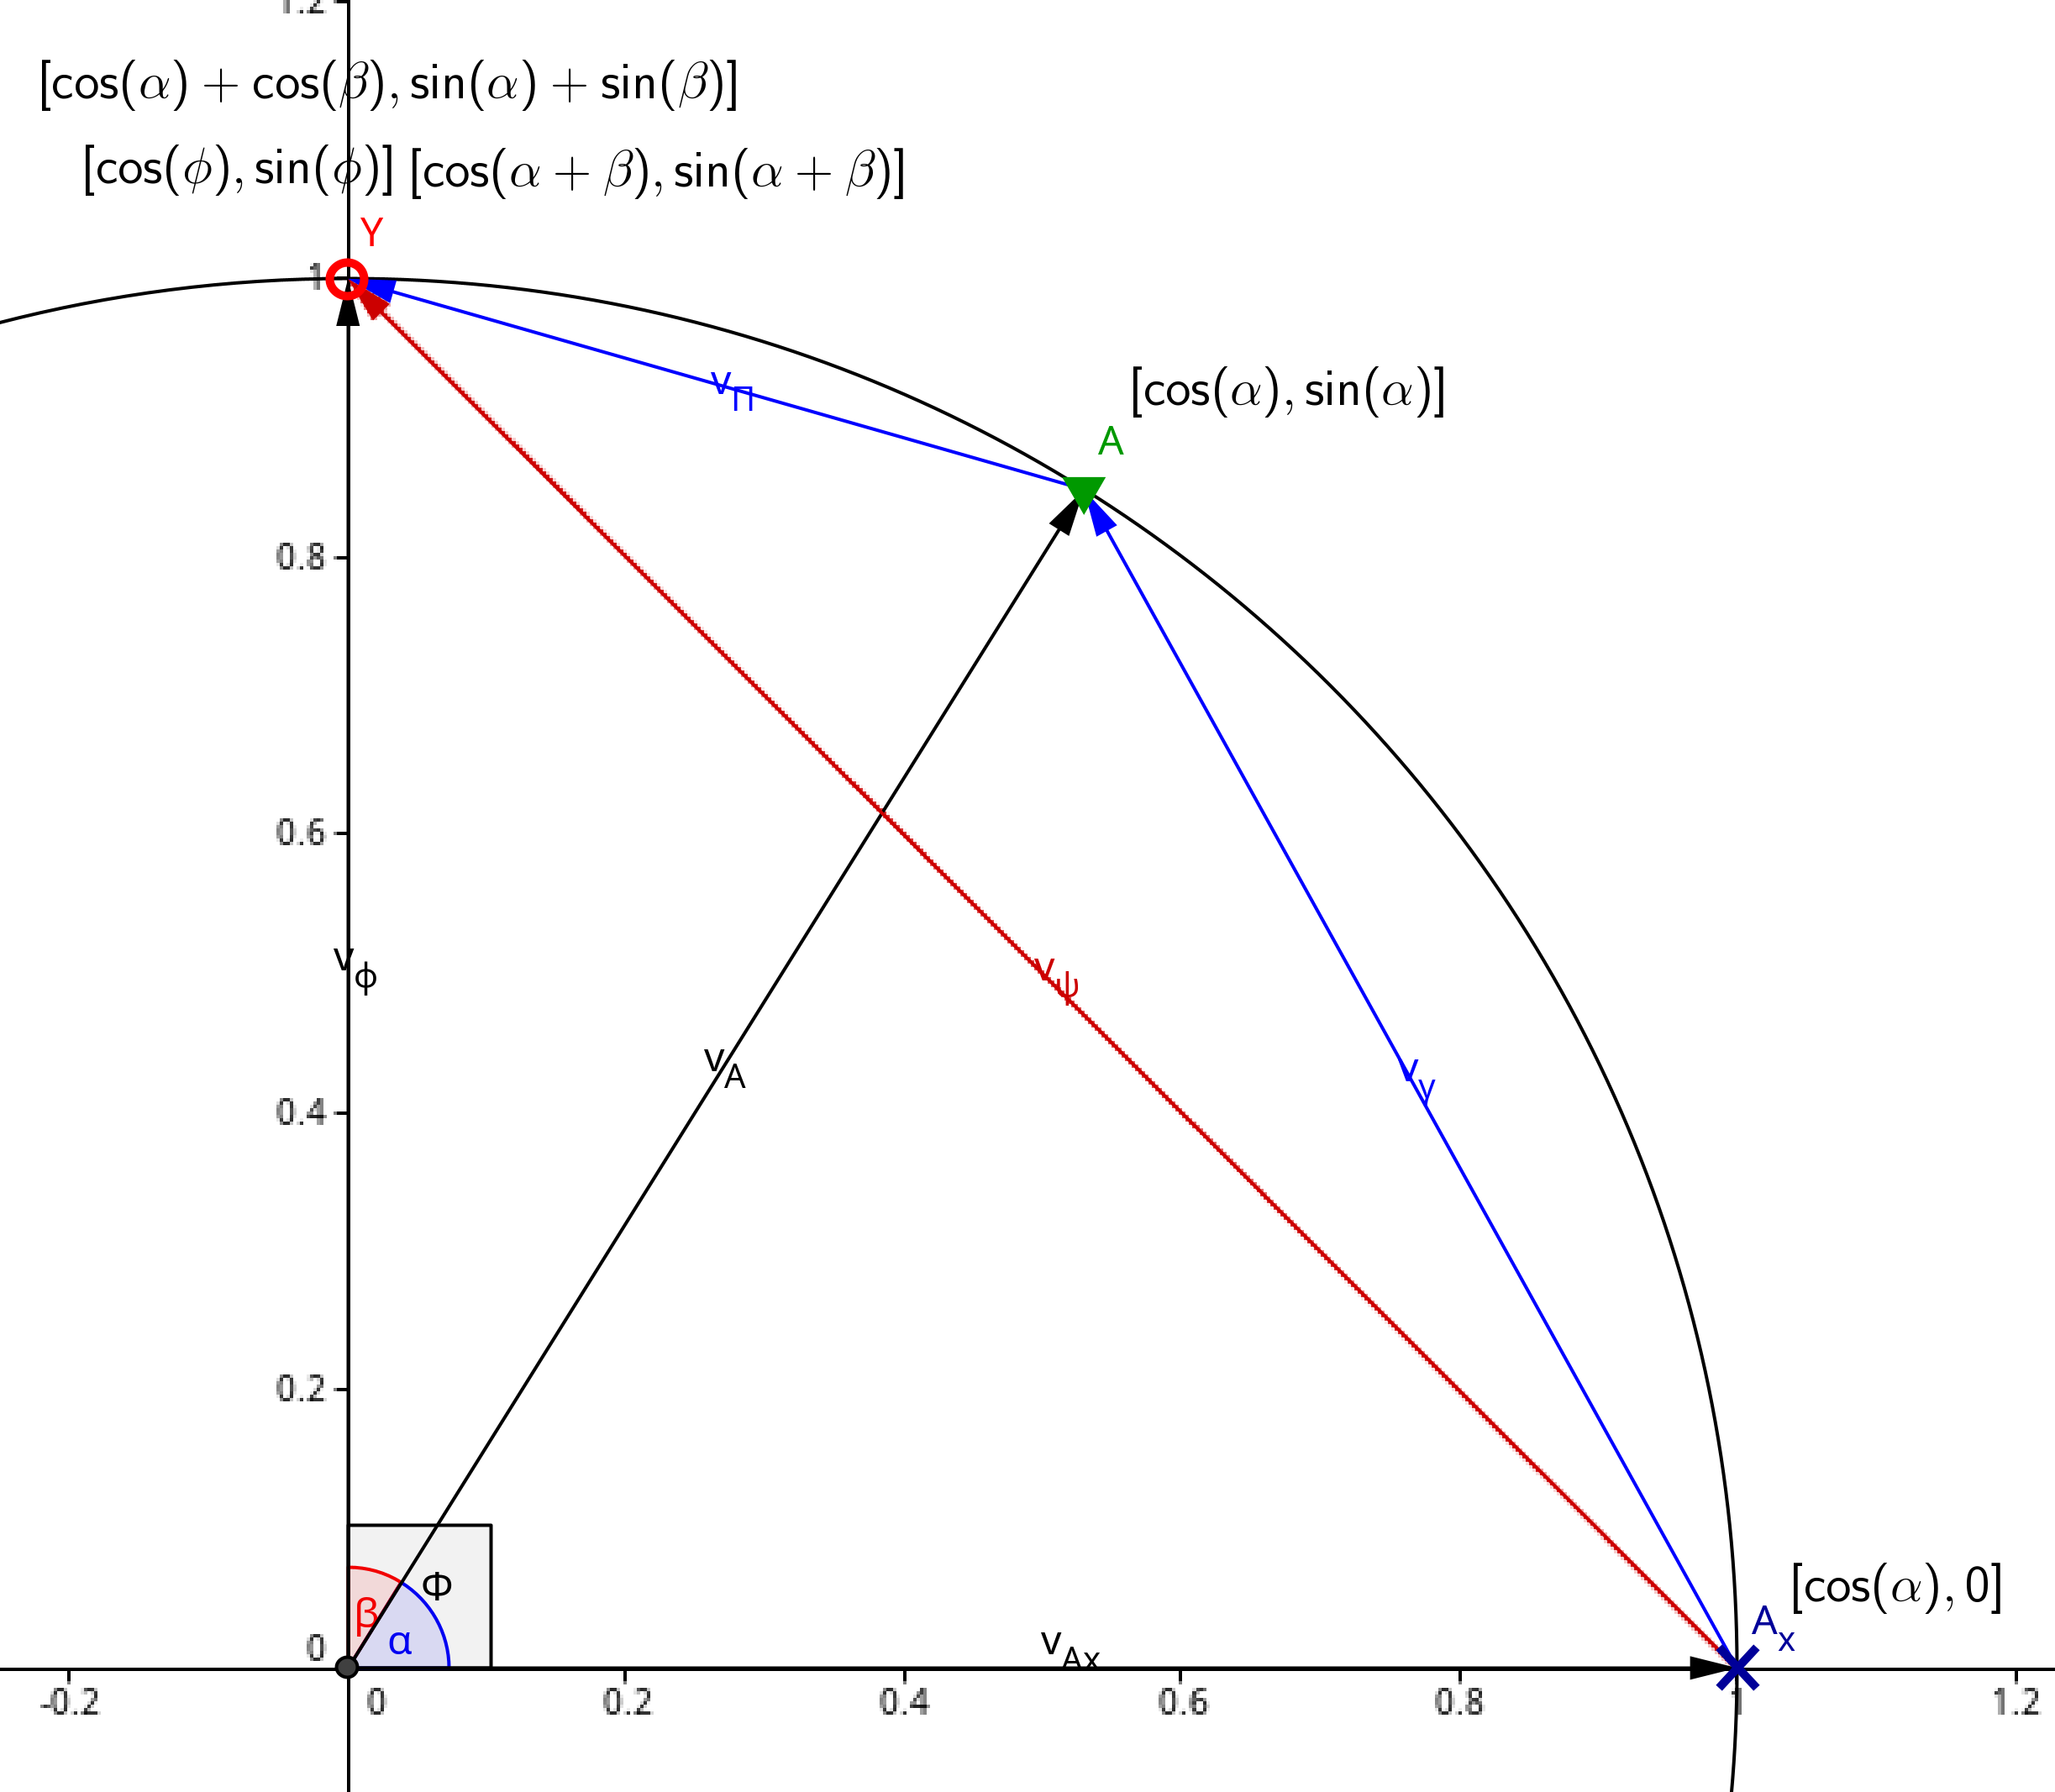
\includegraphics{proof-1.png} 
\\\\ 
\(   
\because
\vec{\Phi} = \vec{\Phi} - \vec{\rho} 
           = (\vec{{\Phi}_x} + \vec{{\Phi}_y}) - \vec{\rho}
            = (\begin{bmatrix}
            \cos{\phi} \\
            0
            \end{bmatrix} + \begin{bmatrix}
            0 \\
            \sin{\phi}
            \end{bmatrix}) - \begin{bmatrix}
            0 \\
            0
            \end{bmatrix} = \begin{bmatrix}
                            \cos{\phi} \\
                            \sin{\phi}
                            \end{bmatrix} \)

\( 
\vec{A} = \vec{A} - \vec{\rho}
             = (\vec{{A}_x} + \vec{{A}_y}) - \vec{\rho}
             = \begin{bmatrix}
                \cos{\alpha} \\
                \sin{\alpha}
                \end{bmatrix}
\)

\(
\vec{\psi} = \vec{\psi} - \vec{\rho}
           = (\vec{{\psi}_x} + \vec{{\psi}_y}) - \vec{{A}_x}
           = \vec{\upsilon} + \vec{\Pi}
\)

\(
\vec{\upsilon} = \vec{\upsilon} - \vec{\rho} 
               = \vec{A} - \vec{A_x}
               = \begin{bmatrix}
                0 \\
                \sin{\alpha}
                \end{bmatrix}
\)

\begin{equation}
\therefore \vec{\Pi} = \vec{\Pi} - \vec{\rho} 
          =  \begin{bmatrix}
            \cos{\beta} \\
            \sin{\beta}
            \end{bmatrix} - \vec{\rho}    
            \\
          = \vec{\Phi} - \vec{A} 
          =  \begin{bmatrix} 
            \cos{\phi} - \cos{\alpha} \\
            \sin{\phi} - \sin{\alpha}
            \end{bmatrix}
\end{equation}


Essentially, in order to compute for $\angle{\beta}$ in an $R^2$ vectorspace, the initial side angle 
must align with the \(+'ve\) direction of the x-axis. 
\\\\
\(\because \vec{\Pi}\) is translated by vector \(\vec{A}\)
of polar coordinates \([\cos{\alpha}, \sin{\alpha}]\) then to
align \(\vec{\Pi}\) to the \(+'ve\) direction of the x-axis, one extra
operation should be attained, a vector translation transformation that 
could be carried on through the preset vector \( \vec{\rho} \):
\\
\(
\vec{\Pi} = \vec{\Pi} - \vec{\rho} \\
          = (\vec{A} + \vec{\Pi}) - \vec{A} \\
          = \begin{bmatrix}
            (\cos{\alpha} + \cos{\beta}) - \cos{\alpha}\\
            (\sin{\alpha} + \sin{\beta}) - \sin{\alpha}
            \end{bmatrix} \\
          = \begin{bmatrix}
            \cos{\beta} \\
            \sin{\beta}
            \end{bmatrix} \\
\)
\\ 
After this transformation, vector \(\vec{\Pi}\) aligns perfectly with the 
\(+'ve\) direction of x-axis rendering computing angle \(\angle{\beta}\) straightforward,
and hence the vector \(\vec{\Pi}\) can be calculated using distance operations: 
\\ 
\(
\vec{\Pi} = \vec{\Pi} - \vec{\rho} \\
          = \vec{\Pi} - \vec{x} \\
          = \begin{bmatrix}
            \cos{\beta} - 1\\
            \sin{\beta} - 0
            \end{bmatrix} \\
\)
\\
\begin{equation}
\because 
\angle{\phi} = \angle{\alpha} + \angle{\beta} \\
\\
\therefore \angle{\beta} = \angle{\phi} - \angle{\alpha} \\
\\
\therefore \vec{\Pi} = \begin{bmatrix}
    \cos{(\phi - \alpha)} - 1\\
    \sin{(\phi - \alpha)}
    \end{bmatrix} \\
\end{equation}
\\
\( \therefore, from (1) and (2), \) we can deduce that the following norms are equal:
\\
\(
\sqrt{{(\cos{\phi} - \cos{\alpha})}^2 + {(\sin{\phi} - \sin{\alpha})}^2} \\
= \sqrt{{(\cos{\phi - \alpha} - 1)}^2 + {(\sin{\phi - \alpha})}^2} 
\\ \cdots \\
2 \cdot (1 - \cos{(\phi - \alpha)}) = 2 \cdot (1 - \cos{\phi}\cdot\cos{\alpha} - \sin{\phi}\cdot\sin{\alpha})
\\ \cdots \\
\)
\specialsubsection{The Cosine Addition Formula}{
\[
\therefore \cos{(\phi - \alpha)} = \cos{\phi}\cdot\cos{\alpha} + \sin{\phi}\cdot\sin{\alpha}
\]
}{red}

}{black}

\specialsubsection{Proof for equation (2) using the Co-Function forumlas}{
\( \because \sin{\theta} = \cos{(\frac{\pi}{2} - \theta)} \); as both cosine and sine functions are co-functions
in the same right-angled triangle or among 2 similar right-angled triangles in a unit circle.
\\\\
\(
\sin{(\phi \pm \alpha)} = \cos{(\frac{\pi}{2} - (\phi \pm \alpha))} 
                      = \cos{((\frac{\pi}{2} - \phi) \mp \alpha)} \\
                      = \cos{(\frac{\pi}{2} - \phi)}\cdot\cos{\alpha} \pm \sin{(\frac{\pi}{2} - \phi)}\cdot\sin{\alpha} \\
                      = \sin{\phi}\cdot\cos{\alpha} \pm \cos{\phi}\cdot\sin{\alpha}
\)
\specialsubsection{The Sine Addition Formula}{
\[
\therefore \sin{(\phi \pm \alpha)} = \sin{\phi}\cdot\cos{\alpha} \pm \cos{\phi}\cdot\sin{\alpha}
\]
}{red}
}{black}

\specialsubsection{Proof for equation (3) using the Tangent fundamental identities}{
\( \because \tan{\theta} = \frac{\sin{\theta}}{\cos{\theta}} \), and from (1) and (2):
\\
\begin{equation} 
\tan{(\phi \pm \alpha)} = \frac{\sin{(\phi \pm \alpha)}}{\cos{(\phi \pm \alpha)}} \\
             = \frac{
                \sin{\phi}\cdot\cos{\alpha} \pm \cos{\phi}\cdot\sin{\alpha}
             }{
                \cos{\phi}\cdot\cos{\alpha} \mp \sin{\phi}\cdot\sin{\alpha}
             }
\end{equation}
\\ 
\( \because \tan{\theta} = \frac{\sin{\theta}}{\cos{\theta}} \\
    \therefore \sin{\theta} = \cos{\theta}\cdot\tan{\theta} 
\)
\\
\(  
\therefore \tan{(\phi \pm \alpha)} =  \frac{
    \tan{\phi}\cdot\cancel{\cos{\phi}\cdot\cos{\alpha}} \pm \cancel{\cos{\phi}\cdot\cos{\alpha}}\cdot\tan{\alpha}
 }{
    \cancel{\cos{\phi}\cdot\cos{\alpha}} \mp \cancel{\cos{\phi}\cdot\cos{\alpha}}\cdot\tan{\alpha}\cdot\tan{\phi}
 }
\)
\\
\specialsubsection{The Tangent Addition Formula}{
\[
    \therefore \tan{(\phi \pm \alpha)} = \frac{
        \tan{\phi} \pm \tan{\alpha}
     }{
        1 \mp \tan{\alpha}\cdot\tan{\phi}
     }
\]
}{red}

}{black}

\specialsubsection{Extra Verification Proofs done differently}{
\specialsubsection{
Verify that: \(
\sin{(\phi + \frac{3\pi}{2})} = - \cos{\phi}
\)
\\
}{

\begin{proof}
\begin{equation} 
\because \sin{(\phi + \frac{3\pi}{2})} = \sin{(\phi + \pi + \frac{\pi}{2})}
                                       = \sin{(\frac{\pi}{2} - (-\phi - \pi))}
\end{equation}

\begin{equation} 
\because \sin{(\frac{\pi}{2} - \alpha)} = \cos{\alpha} 
\end{equation}

\begin{equation}
         \cos{(-\alpha)} = \cos{\alpha}
\end{equation} 


\( \therefore \) from (4), (5), \& (6):
\\
\(
\sin{(\phi + \frac{3\pi}{2})} = \sin{(\frac{\pi}{2} - (-\phi - \pi))} \\
                              = \cos{(-\phi - \pi)} \\
                              = \cos{(-(\phi + \pi))} \\
                              = \cos{(\phi + \pi)} \\
                              = - \cos(\phi)
\)
\end{proof}
}{red}
}{black}

\subsubsection{Co-functions Addition Formulas}

\subsubsection{Double Angle Formulas}

\subsubsection{Half-Angle Formulas}

\subsubsection{Product-Sum Formulas}

\subsubsection{Miscellaneous Equations}



\subsection{Appendix-A: Pythagorean Theorem Prove}

\end{document}

